\documentclass[a4paper, 12pt]{exam}

\makeatletter
\expandafter\providecommand\expandafter*\csname ver@framed.sty\endcsname
{2003/07/21 v0.8a Simulated by exam}
\makeatother

\usepackage{xcolor}
\usepackage{minted}
\usepackage[utf8]{inputenc}
\usepackage{tikz}
\usepackage{caption}
\usepackage{gensymb}
\usepackage{lmodern}
\usepackage{multirow}
\usepackage{booktabs}
\usepackage{array}
\usepackage{adjustbox}
\usepackage{upquote}
\usepackage{amsmath}
\usepackage[hidelinks]{hyperref}
\usetikzlibrary{mindmap,shadows, shapes, arrows, positioning}

\renewcommand{\refname}{\selectfont\normalsize References} 
\pagestyle{headandfoot}

\header{\textbf{Problem Sheet: Trees}}{}{Graph Theory}
\footer{}{Page \thepage\ of \numpages}{}
\marksnotpoints
\pointsinrightmargin

\begin{coverpages}
\end{coverpages}

\begin{document}

\printanswers

\begin{questions}


\question
  Construct all (non-isomorphic) rooted trees of heights from one to four, that have five vertices~\cite{biggs02}.
  Note that there is one of height one, four of height two, three of height three, and one of height four.
  
  \begin{solution}
    \begin{center}
      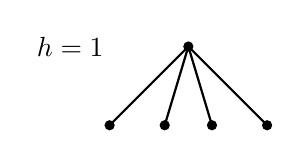
\begin{tikzpicture}
      \begin{scope}[every node/.style={thick,draw,circle,fill,scale=0.3}]
      \node (a) at (1,1) {};
      \node (b) at (0,0) {};
      \node (c) at (0.7,0) {};
      \node (d) at (1.3,0) {};
      \node (e) at (2,0) {};
      \end{scope}
      \begin{scope}[every edge/.style={draw=black,thick}]
      \path (a) edge (b);
      \path (a) edge (c);
      \path (a) edge (d);
      \path (a) edge (e);
      \end{scope}
      \node (l) at (-0.5,1) {$h = 1$};
      \end{tikzpicture}
    \end{center}
    \begin{center}
      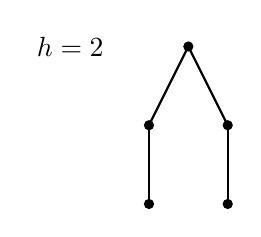
\begin{tikzpicture}
        \begin{scope}[every node/.style={thick,draw,circle,fill,scale=0.3}]
          \node (a) at (0.5,2) {};
          \node (b) at (0,1) {};
          \node (c) at (1,1) {};
          \node (d) at (0,0) {};
          \node (e) at (1,0) {};
        \end{scope}
        \begin{scope}[every edge/.style={draw=black,thick}]
          \path (a) edge (b);
          \path (a) edge (c);
          \path (b) edge (d);
          \path (c) edge (e);
        \end{scope}
        \node (l) at (-1,2) {$h = 2$};
      \end{tikzpicture}
      \hspace{0.4cm}
      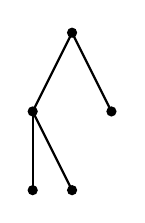
\begin{tikzpicture}
        \begin{scope}[every node/.style={thick,draw,circle,fill,scale=0.3}]
          \node (a) at (0.5,2) {};
          \node (b) at (0,1) {};
          \node (c) at (1,1) {};
          \node (d) at (0,0) {};
          \node (e) at (0.5,0) {};
        \end{scope}
        \begin{scope}[every edge/.style={draw=black,thick}]
          \path (a) edge (b);
          \path (a) edge (c);
          \path (b) edge (d);
          \path (b) edge (e);
        \end{scope}
      \end{tikzpicture}
      \hspace{0.4cm}
      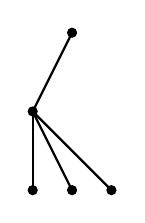
\begin{tikzpicture}
        \begin{scope}[every node/.style={thick,draw,circle,fill,scale=0.3}]
          \node (a) at (0.5,2) {};
          \node (b) at (0,1) {};
          \node (c) at (0,0) {};
          \node (d) at (0.5,0) {};
          \node (e) at (1,0) {};
        \end{scope}
        \begin{scope}[every edge/.style={draw=black,thick}]
          \path (a) edge (b);
          \path (b) edge (c);
          \path (b) edge (d);
          \path (b) edge (e);
        \end{scope}
      \end{tikzpicture}
      \hspace{0.4cm}
      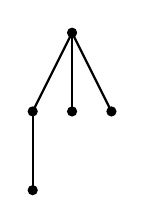
\begin{tikzpicture}
        \begin{scope}[every node/.style={thick,draw,circle,fill,scale=0.3}]
          \node (a) at (0.5,2) {};
          \node (b) at (0,1) {};
          \node (c) at (0.5,1) {};
          \node (d) at (1,1) {};
          \node (e) at (0,0) {};
        \end{scope}
        \begin{scope}[every edge/.style={draw=black,thick}]
          \path (a) edge (b);
          \path (a) edge (c);
          \path (a) edge (d);
          \path (b) edge (e);
        \end{scope}
      \end{tikzpicture}
    \end{center}
    \begin{center}
      \begin{tikzpicture}
        \begin{scope}[every node/.style={thick,draw,circle,fill,scale=0.3}]
        \node (a) at (0.5,3) {};
        \node (b) at (0,2) {};
        \node (c) at (1,2) {};
        \node (d) at (0,1) {};
        \node (e) at (0,0) {};
        \end{scope}
        \begin{scope}[every edge/.style={draw=black,thick}]
        \path (a) edge (b);
        \path (a) edge (c);
        \path (b) edge (d);
        \path (d) edge (e);
        \end{scope}
        \node (l) at (-1,3) {$h = 3$};
      \end{tikzpicture}
      \hspace{0.4cm}
      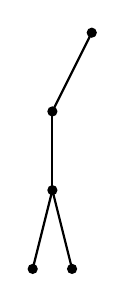
\begin{tikzpicture}
        \begin{scope}[every node/.style={thick,draw,circle,fill,scale=0.3}]
          \node (a) at (0.5,3) {};
          \node (b) at (0,2) {};
          \node (c) at (0,1) {};
          \node (d) at (-0.25,0) {};
          \node (e) at (0.25,0) {};
        \end{scope}
        \begin{scope}[every edge/.style={draw=black,thick}]
          \path (a) edge (b);
          \path (b) edge (c);
          \path (c) edge (d);
          \path (c) edge (e);
        \end{scope}
      \end{tikzpicture}
      \hspace{0.4cm}
      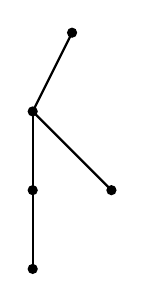
\begin{tikzpicture}
        \begin{scope}[every node/.style={thick,draw,circle,fill,scale=0.3}]
          \node (a) at (0.5,3) {};
          \node (b) at (0,2) {};
          \node (c) at (0,1) {};
          \node (d) at (1,1) {};
          \node (e) at (0,0) {};
        \end{scope}
        \begin{scope}[every edge/.style={draw=black,thick}]
          \path (a) edge (b);
          \path (b) edge (d);
          \path (b) edge (c);
          \path (c) edge (e);
        \end{scope}
      \end{tikzpicture}
    \end{center}
    \begin{center}
      \begin{tikzpicture}
        \begin{scope}[every node/.style={thick,draw,circle,fill,scale=0.3}]
          \node (a) at (0,4) {};
          \node (b) at (0,3) {};
          \node (c) at (0,2) {};
          \node (d) at (0,1) {};
          \node (e) at (0,0) {};
        \end{scope}
        \begin{scope}[every edge/.style={draw=black,thick}]
          \path (a) edge (b);
          \path (b) edge (c);
          \path (c) edge (d);
          \path (d) edge (e);
        \end{scope}
        \node (l) at (-1,3) {$h = 4$};
      \end{tikzpicture}
    \end{center}
  \end{solution}



\question
  Construct two non-isomorphic rooted trees both having twelve vertices, six leaves, and height four~\cite{biggs02}.

  \begin{solution}
    \begin{center}
      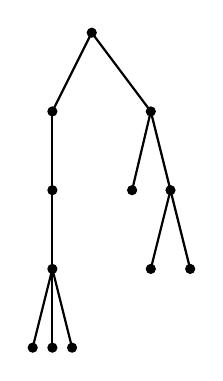
\begin{tikzpicture}
        \begin{scope}[every node/.style={thick,draw,circle,fill,scale=0.3}]
          \node (a) at (-0.5,4) {};
          \node (b) at (-1,3) {};
          \node (c) at (0.25,3) {};
          \node (d) at (-1,2) {};
          \node (e) at (0.0125,2) {};
          \node (f) at (0.5,2) {};
          \node (g) at (-1,1) {};
          \node (h) at (0.25,1) {};
          \node (i) at (0.75,1) {};
          \node (j) at (-1.25,0) {};
          \node (k) at (-1,0) {};
          \node (l) at (-0.75,0) {};
        \end{scope}
        \begin{scope}[every edge/.style={draw=black,thick}]
          \path (a) edge (b);
          \path (a) edge (c);
          \path (b) edge (d);
          \path (c) edge (e);
          \path (c) edge (f);
          \path (d) edge (g);
          \path (f) edge (h);
          \path (f) edge (i);
          \path (d) edge (g);
          \path (g) edge (j);
          \path (g) edge (k);
          \path (g) edge (l);
        \end{scope}
      \end{tikzpicture}
      \hspace{2cm}
      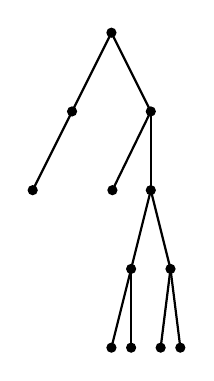
\begin{tikzpicture}
        \begin{scope}[every node/.style={thick,draw,circle,fill,scale=0.3}]
          \node (a) at (0,4) {};
          \node (b) at (-0.5,3) {};
          \node (c) at (0.5,3) {};
          \node (d) at (-1,2) {};
          \node (e) at (0.0125,2) {};
          \node (f) at (0.5,2) {};
          \node (g) at (0.25,1) {};
          \node (h) at (0.75,1) {};
          \node (i) at (0,0) {};
          \node (j) at (0.25,0) {};
          \node (k) at (0.625,0) {};
          \node (l) at (0.875,0) {};
        \end{scope}
        \begin{scope}[every edge/.style={draw=black,thick}]
          \path (a) edge (b);
          \path (a) edge (c);
          \path (b) edge (d);
          \path (c) edge (e);
          \path (c) edge (f);
          \path (f) edge (g);
          \path (f) edge (h);
          \path (g) edge (i);
          \path (g) edge (j);
          \path (h) edge (k);
          \path (h) edge (l);
        \end{scope}
      \end{tikzpicture}
    \end{center}
\end{solution}


\question
  Calculate the minimum height of a ternary rooted tree with eleven leaves.

  \begin{solution}
    We have that $h \leq  \log_m l$.
    Now, $\log_3 11 \approx 2.18$.
    Since the minimum height must be a natural number, and this is a lower bound, we have that the minimum height is 3.
  \end{solution}


\question
  Consider a graph with eight vertices and twelve edges connected such that it can be drawn as a cube.
  Draw this graph, find a spanning tree of it and then high-light the edges on the drawing that are part of the tree~\cite{biggs02}.

  \begin{solution}
    The following is a picture of the graph.
    The edges included in the spanning tree are in red.
    \begin{center}
  	 \begin{adjustbox}{max width=0.6\textwidth}
	  	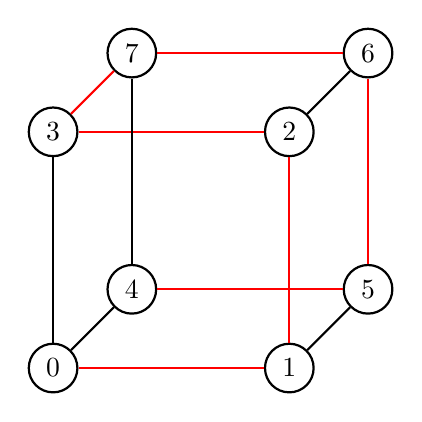
\begin{tikzpicture}
        \begin{scope}[every node/.style={circle,thick,draw}]
          \node (0) at (0,0) {$0$};
          \node (1) at (3,0) {$1$};
          \node (2) at (3,3) {$2$};
          \node (3) at (0,3) {$3$};
          \node (4) at (1,1) {$4$};
          \node (5) at (4,1) {$5$};
          \node (6) at (4,4) {$6$};
          \node (7) at (1,4) {$7$};
        \end{scope}
        \begin{scope}[every edge/.style={draw=black,thick}]
          \path (0) edge[red] (1);
          \path (1) edge[red] (2);
          \path (2) edge[red] (3);
          \path (3) edge (0);
          \path (4) edge[red] (5);
          \path (5) edge[red] (6);
          \path (6) edge[red] (7);
          \path (7) edge (4);
          \path (0) edge (4);
          \path (1) edge (5);
          \path (2) edge (6);
          \path (3) edge[red] (7);
        \end{scope}
  		\end{tikzpicture}
			\end{adjustbox}
		\end{center}
  \end{solution}

\question
  Sketch all sixteen distinct spanning trees of the complete graph $K_4$.

  \begin{solution}
    The complete graph is as follows:
    \begin{center}
      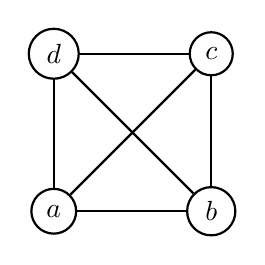
\begin{tikzpicture}
        \begin{scope}[every node/.style={thick,draw,circle}]
          \node (a) at (0,0) {$a$};
          \node (b) at (2,0) {$b$};
          \node (c) at (2,2) {$c$};
          \node (d) at (0,2) {$d$};
        \end{scope}
        \begin{scope}[every edge/.style={draw=black,thick}]
          \path (a) edge (b);
          \path (a) edge (c);
          \path (a) edge (d);
          \path (b) edge (c);
          \path (b) edge (d);
          \path (c) edge (d);
        \end{scope}
      \end{tikzpicture}
    \end{center}

    The spanning trees are then:
    \begin{center}
      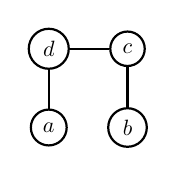
\begin{tikzpicture}
        \begin{scope}[every node/.style={thick,draw,circle,scale=0.8}]
          \node (a) at (0,0) {$a$};
          \node (b) at (1,0) {$b$};
          \node (c) at (1,1) {$c$};
          \node (d) at (0,1) {$d$};
        \end{scope}
        \begin{scope}[every edge/.style={draw=black,thick}]
          %\path (a) edge (b);
          \path (b) edge (c);
          \path (c) edge (d);
          \path (d) edge (a);
        \end{scope}
      \end{tikzpicture}
      \hspace{4mm}
      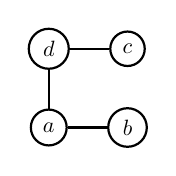
\begin{tikzpicture}
        \begin{scope}[every node/.style={thick,draw,circle,scale=0.8}]
          \node (a) at (0,0) {$a$};
          \node (b) at (1,0) {$b$};
          \node (c) at (1,1) {$c$};
          \node (d) at (0,1) {$d$};
        \end{scope}
        \begin{scope}[every edge/.style={draw=black,thick}]
          \path (a) edge (b);
          %\path (b) edge (c);
          \path (c) edge (d);
          \path (d) edge (a);
        \end{scope}
      \end{tikzpicture}
      \hspace{4mm}
      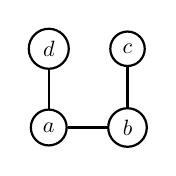
\begin{tikzpicture}
        \begin{scope}[every node/.style={thick,draw,circle,scale=0.8}]
          \node (a) at (0,0) {$a$};
          \node (b) at (1,0) {$b$};
          \node (c) at (1,1) {$c$};
          \node (d) at (0,1) {$d$};
        \end{scope}
        \begin{scope}[every edge/.style={draw=black,thick}]
          \path (a) edge (b);
          \path (b) edge (c);
          %\path (c) edge (d);
          \path (d) edge (a);
        \end{scope}
      \end{tikzpicture}
      \hspace{4mm}
      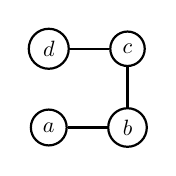
\begin{tikzpicture}
        \begin{scope}[every node/.style={thick,draw,circle,scale=0.8}]
          \node (a) at (0,0) {$a$};
          \node (b) at (1,0) {$b$};
          \node (c) at (1,1) {$c$};
          \node (d) at (0,1) {$d$};
        \end{scope}
        \begin{scope}[every edge/.style={draw=black,thick}]
          \path (a) edge (b);
          \path (b) edge (c);
          \path (c) edge (d);
          %\path (d) edge (a);
        \end{scope}
      \end{tikzpicture}
    \end{center}

    \begin{center}
      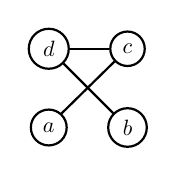
\begin{tikzpicture}
        \begin{scope}[every node/.style={thick,draw,circle,scale=0.8}]
          \node (a) at (0,0) {$a$};
          \node (b) at (1,0) {$b$};
          \node (c) at (1,1) {$c$};
          \node (d) at (0,1) {$d$};
        \end{scope}
        \begin{scope}[every edge/.style={draw=black,thick}]
          %\path (a) edge (b);
          \path (b) edge (d);
          \path (d) edge (c);
          \path (c) edge (a);
        \end{scope}
      \end{tikzpicture}
      \hspace{4mm}
      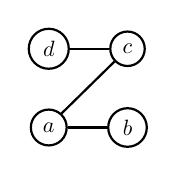
\begin{tikzpicture}
        \begin{scope}[every node/.style={thick,draw,circle,scale=0.8}]
          \node (a) at (0,0) {$a$};
          \node (b) at (1,0) {$b$};
          \node (c) at (1,1) {$c$};
          \node (d) at (0,1) {$d$};
        \end{scope}
        \begin{scope}[every edge/.style={draw=black,thick}]
          \path (a) edge (b);
          %\path (b) edge (d);
          \path (d) edge (c);
          \path (c) edge (a);
        \end{scope}
      \end{tikzpicture}
      \hspace{4mm}
      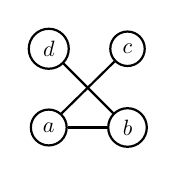
\begin{tikzpicture}
        \begin{scope}[every node/.style={thick,draw,circle,scale=0.8}]
          \node (a) at (0,0) {$a$};
          \node (b) at (1,0) {$b$};
          \node (c) at (1,1) {$c$};
          \node (d) at (0,1) {$d$};
        \end{scope}
        \begin{scope}[every edge/.style={draw=black,thick}]
          \path (a) edge (b);
          \path (b) edge (d);
          %\path (d) edge (c);
          \path (c) edge (a);
        \end{scope}
      \end{tikzpicture}
      \hspace{4mm}
            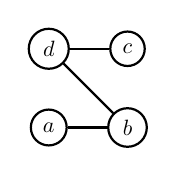
\begin{tikzpicture}
        \begin{scope}[every node/.style={thick,draw,circle,scale=0.8}]
          \node (a) at (0,0) {$a$};
          \node (b) at (1,0) {$b$};
          \node (c) at (1,1) {$c$};
          \node (d) at (0,1) {$d$};
        \end{scope}
        \begin{scope}[every edge/.style={draw=black,thick}]
          \path (a) edge (b);
          \path (b) edge (d);
          \path (d) edge (c);
          %\path (c) edge (a);
        \end{scope}
      \end{tikzpicture}
    \end{center}

    \begin{center}
      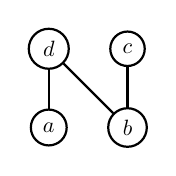
\begin{tikzpicture}
        \begin{scope}[every node/.style={thick,draw,circle,scale=0.8}]
          \node (a) at (0,0) {$a$};
          \node (b) at (1,0) {$b$};
          \node (c) at (1,1) {$c$};
          \node (d) at (0,1) {$d$};
        \end{scope}
        \begin{scope}[every edge/.style={draw=black,thick}]
          \path (a) edge (d);
          \path (d) edge (b);
          \path (b) edge (c);
          %\path (c) edge (a);
        \end{scope}
      \end{tikzpicture}
      \hspace{4mm}
      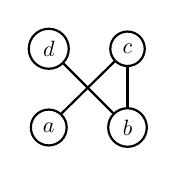
\begin{tikzpicture}
        \begin{scope}[every node/.style={thick,draw,circle,scale=0.8}]
          \node (a) at (0,0) {$a$};
          \node (b) at (1,0) {$b$};
          \node (c) at (1,1) {$c$};
          \node (d) at (0,1) {$d$};
        \end{scope}
        \begin{scope}[every edge/.style={draw=black,thick}]
          %\path (a) edge (d);
          \path (d) edge (b);
          \path (b) edge (c);
          \path (c) edge (a);
        \end{scope}
      \end{tikzpicture}
      \hspace{4mm}
      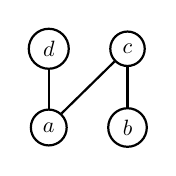
\begin{tikzpicture}
        \begin{scope}[every node/.style={thick,draw,circle,scale=0.8}]
          \node (a) at (0,0) {$a$};
          \node (b) at (1,0) {$b$};
          \node (c) at (1,1) {$c$};
          \node (d) at (0,1) {$d$};
        \end{scope}
        \begin{scope}[every edge/.style={draw=black,thick}]
          \path (a) edge (d);
          %\path (d) edge (b);
          \path (b) edge (c);
          \path (c) edge (a);
        \end{scope}
      \end{tikzpicture}
      \hspace{4mm}
      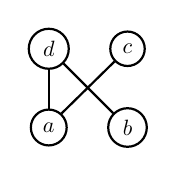
\begin{tikzpicture}
        \begin{scope}[every node/.style={thick,draw,circle,scale=0.8}]
          \node (a) at (0,0) {$a$};
          \node (b) at (1,0) {$b$};
          \node (c) at (1,1) {$c$};
          \node (d) at (0,1) {$d$};
        \end{scope}
        \begin{scope}[every edge/.style={draw=black,thick}]
          \path (a) edge (d);
          \path (d) edge (b);
          %\path (b) edge (c);
          \path (c) edge (a);
        \end{scope}
      \end{tikzpicture}
    \end{center}

    \begin{center}
      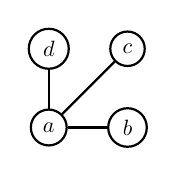
\begin{tikzpicture}
        \begin{scope}[every node/.style={thick,draw,circle,scale=0.8}]
          \node (a) at (0,0) {$a$};
          \node (b) at (1,0) {$b$};
          \node (c) at (1,1) {$c$};
          \node (d) at (0,1) {$d$};
        \end{scope}
        \begin{scope}[every edge/.style={draw=black,thick}]
          \path (a) edge (b);
          \path (a) edge (c);
          \path (a) edge (d);
        \end{scope}
      \end{tikzpicture}
      \hspace{4mm}
      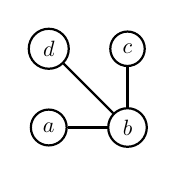
\begin{tikzpicture}
        \begin{scope}[every node/.style={thick,draw,circle,scale=0.8}]
          \node (a) at (0,0) {$a$};
          \node (b) at (1,0) {$b$};
          \node (c) at (1,1) {$c$};
          \node (d) at (0,1) {$d$};
        \end{scope}
        \begin{scope}[every edge/.style={draw=black,thick}]
          \path (b) edge (a);
          \path (b) edge (c);
          \path (b) edge (d);
        \end{scope}
      \end{tikzpicture}
      \hspace{4mm}
            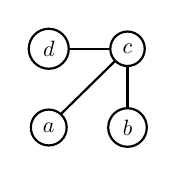
\begin{tikzpicture}
        \begin{scope}[every node/.style={thick,draw,circle,scale=0.8}]
          \node (a) at (0,0) {$a$};
          \node (b) at (1,0) {$b$};
          \node (c) at (1,1) {$c$};
          \node (d) at (0,1) {$d$};
        \end{scope}
        \begin{scope}[every edge/.style={draw=black,thick}]
          \path (c) edge (a);
          \path (c) edge (b);
          \path (c) edge (d);
        \end{scope}
      \end{tikzpicture}
      \hspace{4mm}
            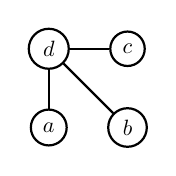
\begin{tikzpicture}
        \begin{scope}[every node/.style={thick,draw,circle,scale=0.8}]
          \node (a) at (0,0) {$a$};
          \node (b) at (1,0) {$b$};
          \node (c) at (1,1) {$c$};
          \node (d) at (0,1) {$d$};
        \end{scope}
        \begin{scope}[every edge/.style={draw=black,thick}]
          \path (d) edge (a);
          \path (d) edge (b);
          \path (d) edge (c);
        \end{scope}
      \end{tikzpicture}
    \end{center}
  \end{solution}

\end{questions}

\bibliographystyle{plain}
\bibliography{bibliography}
\end{document}
